\subsection{Methodology}
\begin{frame}
    \frametitle{Transition analysis doesn't tell the full story}
    \begin{itemize}
        \item From the transition analysis we learned how changing which 
              reactor is predominantly built affects the material 
              requirements
        \item There are so many more parameters and assumptions in the scenario modeled
        \item We can use sensitivity analysis to see the effect of other model 
              parameters on the material requirements
    \end{itemize}
\end{frame}

\begin{frame}
    \frametitle{Sensitivity analysis provides insight into how decisions affect material needs}
    \begin{itemize}
        \item Vary a single parameter at a time and observe the output
        \item Helps to identify different relationships about the transition
        \item Couple \Cyclus with Dakota \cite{adams_dakota_2019}, model 
              variations in Scenario 7
    \end{itemize}
    \begin{columns}
        \column[t]{5cm}<2->
        Model inputs (parameters)
        \begin{itemize}
            \item Transition start time, January 2025-January 2040 
            \item LWR lifetime: percent of LWR fleet operating 
                  for 80 years, 0-50\%
            \item Build share of each advanced reactor, 0-50\%
            \item \gls{MMR} \& Xe-100 discharge burnup
        \end{itemize}

        \column[t]{5cm}<3->
        Model outputs (metrics, material requirements)
        \begin{itemize}
            \item Total fuel mass 
            \item HALEU mass
            \item Total \gls{SWU}
            \item SWU to produce HALEU
            \item Feed to produce HALEU
            \item \gls{SNF} mass
        \end{itemize}
    \end{columns}
\end{frame}

\begin{frame}
    \frametitle{Adjust deployment when varying the build share}
    \begin{columns}
        \column{4.5cm}
            \begin{itemize}
                \item Deploy the specified reactor first to meet the build share
                \item Deploy the other reactors using the previous scheme (largest 
                      to smallest power output) to meet the remaining demand
                \item Deployment schedule is given to \Cyclus
            \end{itemize}

        \column{6cm}
            \begin{figure}
                \centering 
                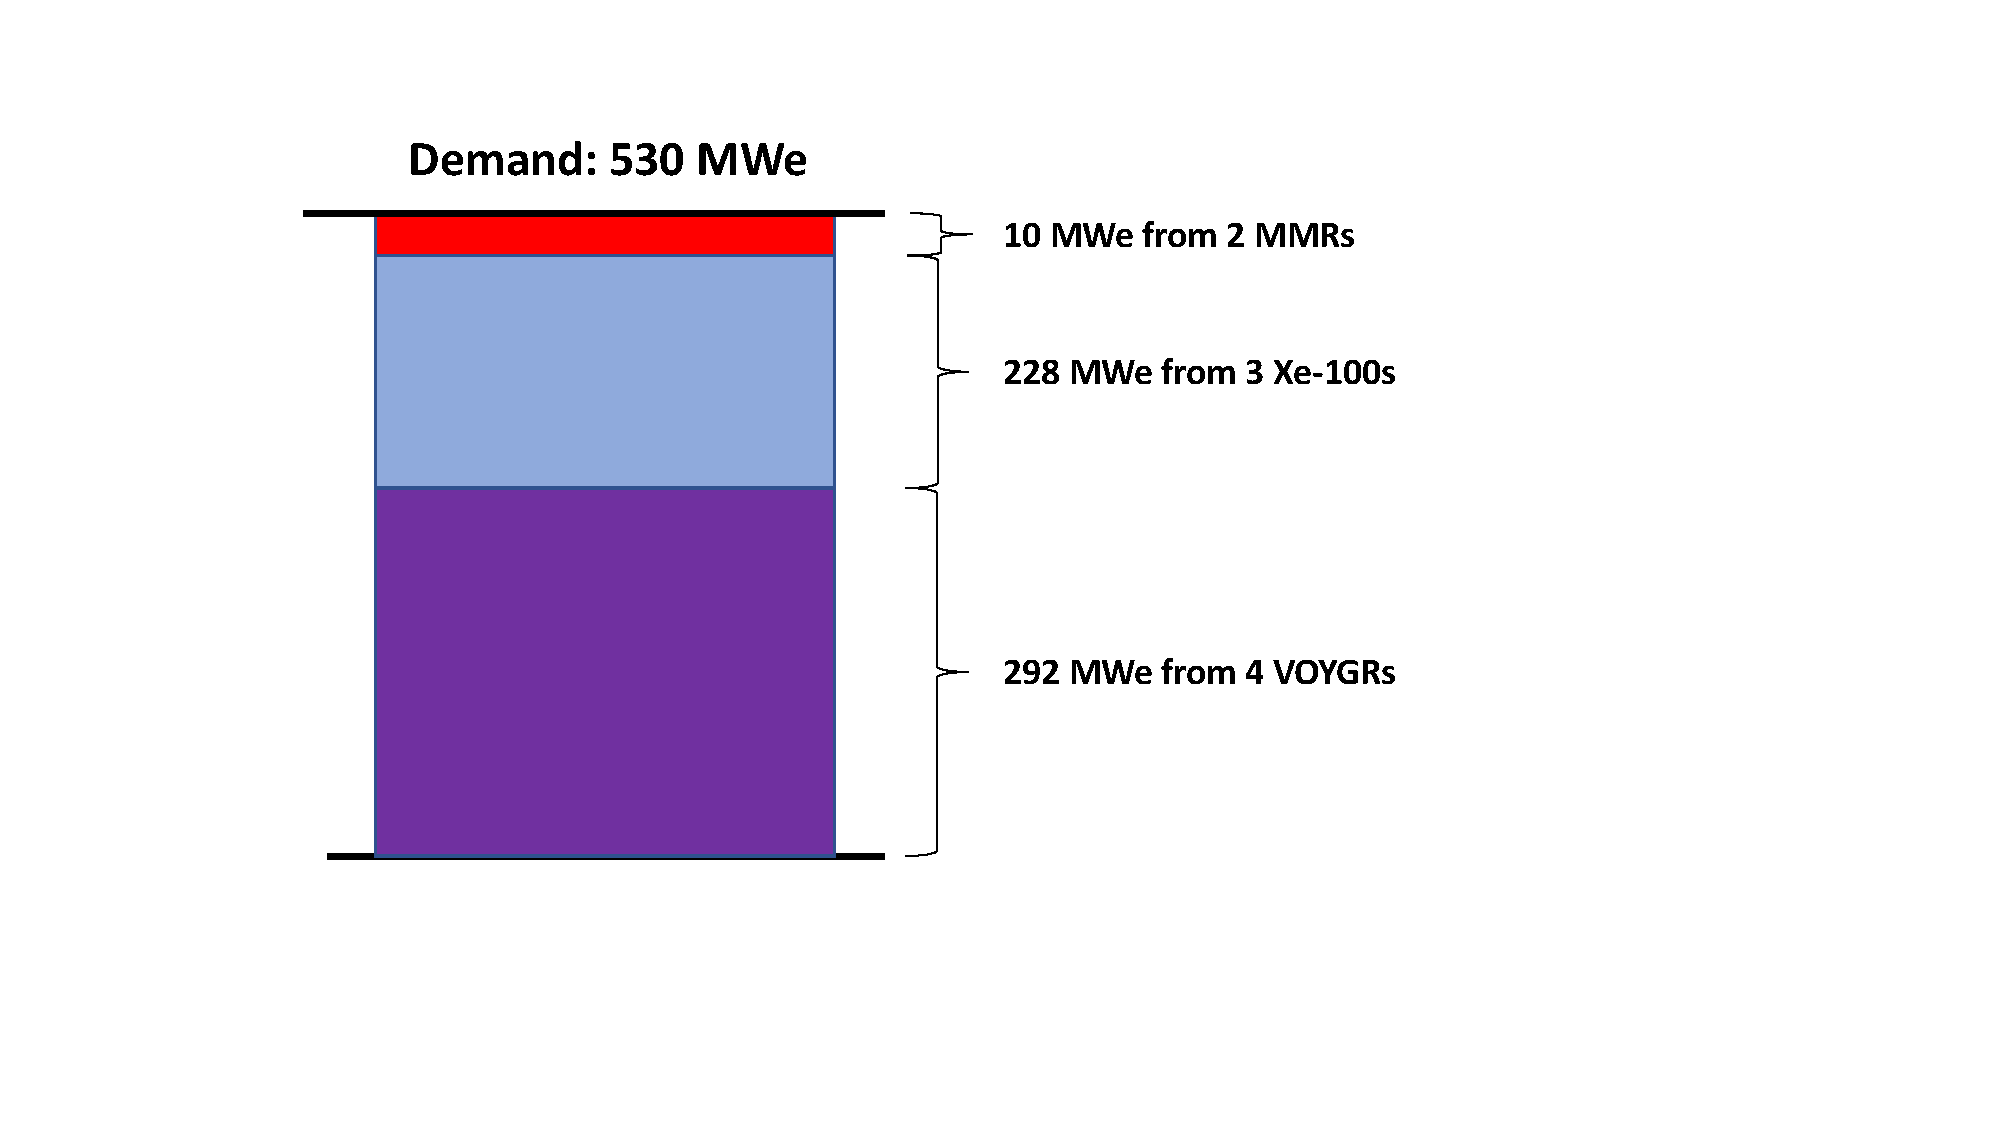
\includegraphics[scale=0.33, trim=100 100 50 50,clip]{VOYGR_build_share.pdf}
                \caption{Deployment of advanced reactors to meet 
                a demand of 530 MWe and a 50\% VOYGR build share.}
                \label{fig:build_share_deployment}
            \end{figure}
    \end{columns}
\end{frame}